\documentclass[a4paper,UKenglish,cleveref,autoref,english]{lipics-v2019}
%This is a template for producing LIPIcs articles. 
%See lipics-manual.pdf for further information.
%for A4 paper format use option "a4paper", for US-letter use option
%"letterpaper" 
%for british hyphenation rules use option "UKenglish", for american
%hyphenation rules use option "USenglish" 
%for section-numbered lemmas etc., use "numberwithinsect"
%for enabling cleveref support, use "cleveref"
%for enabling cleveref support, use "autoref"

%helpful if your graphic files are in another directory
\graphicspath{
  {../svg/}
  {./plot/UFS-alg/}
  {./plot/2D-UFS/}
  {./plot/avg-alg-sched/}
  {../aux}
  {./aux}
}

\bibliographystyle{plainurl}% the mandatory bibstyle

\title{\texttt{NPM-BUNDLE}: Non-Preemptive Multitask Scheduling for
  Jobs with \texttt{BUNDLE}-based Thread-Level Scheduling}

%optional, please use if title is longer than one line
\titlerunning{\texttt{NPM-BUNDLE}: Non-Preemptive Multitask \texttt{BUNDLE}}

\author{Corey Tessler}
       {Wayne State University, Detroit, Michigan, United States}
       {corey.tessler@wayne.edu}
       {}
       {}

\author{Nathan Fisher}
       {Wayne State University, Detroit, Michigan, United States}
       {fishern@wayne.edu}
       {}
       {}

%TODO mandatory. First: Use abbreviated first/middle names. Second
%(only in severe cases): Use first author plus 'et al.'        
\authorrunning{C. Tessler and N. Fisher}

%TODO mandatory, please use full first names. LIPIcs license is
%"CC-BY";  http://creativecommons.org/licenses/by/3.0/ 
\Copyright{Corey Tessler and Nathan Fisher}

%TODO mandatory: Please choose ACM 2012 classifications from
%https://dl.acm.org/ccs/ccs_flat.cfm
\ccsdesc{Computer systems organization~Real-time systems}
\ccsdesc{Software and its engineering~Real-time schedulability}

%TODO mandatory; please add comma-separated list of keywords
\keywords{Scheduling algorithms, Cache Memory, Multi-threading,
  Static Analysis}

%optional, e.g. invited paper
\category{}

%optional, e.g. full version hosted on arXiv, HAL, or other
%respository/website \relatedversion{A full version of the paper is
%available at %\url{...}.} 
\relatedversion{}

%optional, e.g. related research data, source code, ... hosted on a
%repository like zenodo, figshare, GitHub, ...
\supplement{}

%\funding{(Optional) general funding statement \dots}%optional, to
%capture a funding statement, which applies to all authors. Please
%enter author specific funding statements as fifth argument of the
%\author macro.
\funding{The research presented in this paper was supported
  by the National Science Foundation under Grant Nos. CNS-1618185 and
  IIS-1724227.}

\nolinenumbers %uncomment to disable line numbering

%\hideLIPIcs  %uncomment to remove references to LIPIcs series (logo,
%DOI, ...), e.g. when preparing a pre-final version to be uploaded to
%arXiv or another public repository 

%Editor-only macros:: begin (do not touch as%author) %%
\EventEditors{Sophie Quinton}
\EventNoEds{1}
\EventLongTitle{31st Euromicro Conference on Real-Time Systems (ECRTS 2019)}
\EventShortTitle{ECRTS 2019}
\EventAcronym{ECRTS}
\EventYear{2019}
\EventDate{July 9--12, 2019}
\EventLocation{Stuttgart, Germany}
\EventLogo{}
\SeriesVolume{133}
\ArticleNo{19}
%%%%%%%%%%%%%%%%%%%%%%%%%%%%%%%%%%%%%%%%%%%%%%%%%%%%%%


% %%%%%%%%%%%%%%%%%%%%%%%%%%%%%%%%%%%%%%%%%%%%%%%%%%%%%%%%%%%%%%%%%%%%%%%%%%%%%
% Packages not supplied by LIPICS
%
% There are code listings, but no algorithm or pseudocode package 
\usepackage{algorithm,setspace}
\usepackage{algpseudocode}
\usepackage{relsize}
\usepackage{amsmath}
\usepackage{wrapfig} % Flowing text around figures.
\usepackage{subcaption} % subfigure is deprecated
\usepackage{gnuplottex}
% \usepackage{multirow} % For entries spanning multiple rows in tables
% %%%%%%%%%%%%%%%%%%%%%%%%%%%%%%%%%%%%%%%%%%%%%%%%%%%%%%%%%%%%%%%%%%%%%%%%%%%%%

\newtheorem{prop}{Property}
\DeclareMathOperator{\argmax}{argmax}

\addtolength{\parskip}{-0.5mm}
\setlength{\textfloatsep}{0.1cm}
\setlength{\intextsep}{2pt}
\captionsetup{skip=4pt}
\setlength{\belowcaptionskip}{1pt}

\newcommand{\bundlep}{\texttt{BUNDLEP}}
\newcommand{\bundle}{\texttt{BUNDLE}}

\begin{document}
\maketitle

%%%%%%%%%%%%%%%%%%%%%%%%%%%%%%%%%%%%%%%%%%%%%%%%%%%%%%%%%%%%%%%%%%%%%%
% Macros and Notation
% Macros for commonly used symbols and functions to ensure that their
% use remains consistent.
%%%%%%%%%%%%%%%%%%%%%%%%%%%%%%%%%%%%%%%%%%%%%%%%%%%%%%%%%%%%%%%%%%%%%%

% Block Reload Time - \BRT
\newcommand{\BRT}{\ensuremath{\mathbb{B}}}
% Cycles Per Instruction - \CPI
\newcommand{\CPI}{\ensuremath{\mathbb{I}}}
% Task Set - \tasks
\newcommand{\tasks}{\ensuremath{\tau}}
% Individual Task - \task{n}
\newcommand{\task}[1]{\ensuremath{\tau_{#1}}}
% Minimum inter-arrival time - \period{n}
\newcommand{\period}[1]{\ensuremath{p_{#1}}}
% Relative deadline - \deadline{n}
\newcommand{\deadline}[1]{\ensuremath{d_{#1}}}
% Absolute deadline - \Deadline{n}
\newcommand{\Deadline}[1]{\ensuremath{D_{#1}}}
% Number of threads released with each job of task n - \taskthreads{n}
\newcommand{\taskthreads}[1]{\ensuremath{m_{#1}}}
% WCET - \wcet{n}{m}
%    n - task number
%    m - number of threads
\newcommand{\wcet}[2]{\ensuremath{c_{#1}{(#2)}}}
% Object of execution - \object{i}
\newcommand{\object}[1]{\ensuremath{o_{#1}}}
% SLACK - \slack{${D_i}$}
\newcommand{\slack}[1]{\text{\sc{slack}(#1)}}
% DBF - \dbf{\tau_i}{\Deadline{k}}
\newcommand{\dbf}[2]{\text{\sc{dbf}(#1,#2)}}
% Hyper Period - \hp
\newcommand{\hp}{\ensuremath{P}}

% Superior indicator  - \supp{\tasks{}}
\newcommand{\supi}[1]{\ensuremath{\hat{#1}}}
% Superior Task Set - \supset
\newcommand{\supts}{\ensuremath{\hat{\tau}}}
% Anterior Task Set - \ants
\newcommand{\ants}{\ensuremath{\hat{\tau}}}
% Anterior task - \ant{i}
\newcommand{\ant}[1]{\ensuremath{\hat{\task{}}_#1}}

% Maximum Period and Relative Deadline Difference -
\newcommand{\pd}{\ensuremath{\Delta_{max}}}
% DIVIDE procedure \algdivide{t}{q}
%    t - the task
%    q - non preemptive chunk size
%    \algdivide{\task{i}}{q}
\newcommand{\algdivide}[2]{\text{\sc{divide}(#1,#2)}}
% DIVIDE as a name
\newcommand{\texdivide}{\text{\sc{divide}}}
% Partial tasks
%    i - the task being divided
%
\newcommand{\Partial}[1]{\ensuremath{\Phi_{#1}}}

% Growth Factor
\newcommand{\GFactor}{\ensuremath{\mathbb{F}}}

% NP-CHUNKS
\newcommand{\npchunks}{\text{\sc{np-chunks}}}
% BNG
\newcommand{\bng}{\text{\sc{bnc}}}
% TPJ
\newcommand{\tpj}{\text{\sc{tpj}}}

% S values
\newcommand{\stpj}{\ensuremath{s^{\text{\sc{tpj}}}}}

%
% To be overridden by over-one.tex
% 
\newcommand{\totalTaskSets}{-}
% Total number of task sets when \tau^1 utilization > 1
\newcommand{\totalOverOne}{-}
% Total number of OverOne task sets TPJ could schedule
\newcommand{\totalOOTPJ}{-}
% OverOne Ratio
\newcommand{\ratioOverOne}{-}
% TPJ ratio
\newcommand{\ratioOOTPJ}{-}
%
% end override
%

%%%%%%%%%%%%%%%%%%%%%%%%%%%%%%%%%%%%%%%%%%%%%%%%%%%%%%%%%%%%%%%%%%%%%%
% Abstract
%%%%%%%%%%%%%%%%%%%%%%%%%%%%%%%%%%%%%%%%%%%%%%%%%%%%%%%%%%%%%%%%%%%%%%
\begin{abstract}

  The \bundle{} and \bundlep{} scheduling algorithms are cache-cognizant
  thread-level scheduling algorithms and associated worst case
  execution time and cache overhead (WCETO) techniques for hard
  real-time multi-threaded tasks. The \texttt{BUNDLE}-based approaches
  utilize the inter-thread cache benefit to reduce WCETO values for 
  jobs. Currently, the \texttt{BUNDLE}-based approaches are limited to
  scheduling a single task. This work aims to expand the applicability
  of \texttt{BUNDLE}-based scheduling to multiple task multi-threaded
  task sets.

  \texttt{BUNDLE}-based scheduling leverages knowledge of potential
  cache conflicts to selectively preempt one thread in favor of
  another from the same job. This thread-level preemption is a
  requirement for the run-time behavior and WCETO calculation to
  receive the benefit of \texttt{BUNDLE}-based approaches. This work
  proposes scheduling \texttt{BUNDLE}-based jobs non-preemptively
  according to the earliest deadline first (EDF) policy. Jobs are
  forbidden from preempting one another, while threads within a job
  are allowed to preempt other threads.

  An accompanying schedulability test is provided, named Threads Per
  Job (\tpj{}). \tpj{} is a novel schedulability test, input is a task
  set specification which may be transformed (under certain
  restrictions); dividing threads among tasks in an effort to find
  a feasible task set. Enhanced by the flexibility to transform task
  sets and taking advantage of the inter-thread cache benefit, the
  evaluation shows \tpj{} scheduling task sets fully preemptive EDF
  cannot. 
  
\end{abstract}

%%%%%%%%%%%%%%%%%%%%%%%%%%%%%%%%%%%%%%%%%%%%%%%%%%%%%%%%%%%%%%%%%%%%%%
% Introduction
%%%%%%%%%%%%%%%%%%%%%%%%%%%%%%%%%%%%%%%%%%%%%%%%%%%%%%%%%%%%%%%%%%%%%%
\section{Introduction}

Hard real-time multi-threaded task systems which incorporate cache
memory, must account for the variation in execution time and cache
related preemption delays found in single-threaded task systems. For
multi-threaded task systems, the complexity of cache interactions is
increased due to thread-level cache interference and preemptions.
Worst-case execution time (WCET) and schedulability analysis of hard
real-time multi-threaded tasks commonly treat threads
independently~\cite{Pellizzoni:2011} or utilize cache management
techniques~\cite{Ward:2013} to limit the cache interference. 

Analysis techniques focusing on independent treatment or
limiting of cache interference exclude the possible benefit of
caches. Multi-threaded tasks may benefit from caches. By virtue of
sharing the same address space one thread of a task may cache values
on behalf of another reducing the total execution time to complete
both. This positive effect is referred to as the
\emph{inter-thread cache benefit}~\cite{Tessler:2016}. 

Currently, only the \bundle{}~\cite{Tessler:2016} and
\bundlep{}~\cite{Tessler:2018} analysis techniques and cache
congnizant thread-level scheduling algorithms incorporate the
inter-thread cache benefit into WCET and schedulability
analysis. These \texttt{BUNDLE}-based approaches are currently limited
to a \underline{single} multi-threaded task. The primary focus of this
work is to provide a scheduling algorithm and schedulability test for
multi-threaded task sets with multiple tasks, where individual jobs
utilize \texttt{BUNDLE}-based scheduling. As the first scheduling
algorithm to incorporate \texttt{BUNDLE}-based thread-level
scheduling, a non-preemptive algorithm was chosen to avoid necessary
modifications to \bundle{} and \bundlep{}. Non-preemptive EDF was
selected as the task-level scheduler, as the proposed schedulability
test presented in Section~\ref{sec:schedulability} is based upon
Baruah's limited-preemption for EDF~\cite{Baruah:2005} algorithm. 

An additional consideration is made for alternative approaches and
the unforeseen benefits to schedulability of thread-level schedulers
of non-preemptive multi-threaded jobs. If the WCET of jobs can be
expressed as a strictly increasing discrete concave function of the
number of threads per job, the schedulability test developed for this
work applies without modification to the \texttt{BUNDLE}-based
approaches or non-preemptive EDF scheduling. 

In the following sections, the key contributions are:
\begin{enumerate}
  \item A model of hard real-time multi-threaded tasks which is
    compatible with existing single-threaded models, where tasks sets
    may be transformed through division of threads.
  \item A schedulability test named Threads Per Job (\tpj{}) that provides a
    schedulability result and transformed feasible task set if the
    specified task set could not be scheduled non-preemptively.
  \item Proof of \tpj{}'s optimality with respect to non-preemptive
    multi-threaded feasibility.
  \item An improvement to Baruah's~\cite{Baruah:2005}
    non-preemptive chunk algorithm, increasing chunk sizes.
  \item An evaluation of over 500,000 task sets, comparing the
    schedulability ratio of \tpj{} to those of non-preemptive and
    (limited) preemptive EDF, with an accompanying implementation available for
    download~\cite{NPM-Artifact:2019}.
\end{enumerate}

These contributions are presented following the related
research of Section~\ref{sec:related}. Section~\ref{sec:model}
introduces the proposed model, application of non-preemptive EDF
scheduling for thread-level schedulers, and the requirements of task
transformation. Section~\ref{sec:schedulability} introduces then
improves upon the non-preemptive chunk algorithm~\cite{Baruah:2005},
followed by the \tpj{} schedulability algorithm and proof of
feasibility. Section~\ref{sec:eval} compares the schedulability ratio
of \tpj{} to other non-preemptive and preemptive scheduling
algorithms, before concluding with Section~\ref{sec:conclusion}. 

%%%%%%%%%%%%%%%%%%%%%%%%%%%%%%%%%%%%%%%%%%%%%%%%%%%%%%%%%%%%%%%%%%%%%%
% Related Work
%%%%%%%%%%%%%%%%%%%%%%%%%%%%%%%%%%%%%%%%%%%%%%%%%%%%%%%%%%%%%%%%%%%%%%
\section{Discussion of Related Research}
\label{sec:related}

\noindent
{\bf Single-Threaded Tasks:}  The challenge of dealing with the
non-uniformity of execution times in real-time systems due to cache
misses or hits has received considerable attention~\cite{Wilhelm:2008,Theiling:2000}. In
particular, much of the 
prior real-time systems work on understanding caches vis-\`{a}-vis scheduling has focused upon the contention in the
cache due to tasks preempting each other.  Roughly speaking, a large
majority of this research can be classified into two categories:
\emph{cache-related preemption delay (CRPD) analysis} and
\emph{deferred/limited-preemption scheduling}. 
The goal of CRPD analysis is to bound the number of cache blocks of a
task that need to be reloaded due to evictions caused by a preempting
task.  The foundation of CRPD analysis is the development of
techniques for counting and bounding the number of blocks affected by
preemption; this is achieved by categorizing a task's cache blocks
into sets of useful cache blocks (UCBs) or evicting cache block
(ECBs)~\cite{Lee:1998,Tomiyama:2000}.  The size of these sets can be
used as an upper bound on the cache cost of a preemption.  Subsequent
research based upon this UCB and ECB categorization has refined these
sets and incorporated the CRPD analysis into schedulability
analysis~\cite{Altmeyer:2012,Altmeyer:2011,Altmeyer:2011b,Negi:2003,
  Staschulat:2005, Tan:2004}. 
However, please note that these CRPD approaches only quantify the
cache effect of preemption into existing scheduling approaches and do not
change any scheduling decision based upon the knowledge of
preemption. 

In limited/deferred-preemption scheduling, a higher-priority task may
preempt a lower-priority task only when some condition is satisfied.
The overall effect of deferring or limiting preemptions is to reduce
the number of times a task may be preempted during its execution.  The
hope is that by limiting the number of preemptions this will lead to a
decrease in the execution time of job due to the cache overhead of
preemption.  Different conditions for deferring preemptions have been
considered.  The fixed preemption-point approach~\cite{Burns:1995}
selects specific locations in a task code that are most appropriate
for the program but preserve the system schedulability.  The
preemption-threshold scheduling approach~\cite{Wang:1999} sets a
threshold that only task with higher-priority than this threshold may
preempt a currently-executing lower priority task.  The floating
preemption-point model~\cite{Baruah:2005,Marinho:2012} computes the
maximum time duration that a lower-priority task may delay the
preemption of a higher-priority task.  Each of the deferred preemption
approaches have been shown to limit the number of preemptions but do
not incorporate the CRPD overhead cost in its decision on how to defer
preemption. 

More recently, a line of research has emerged to combine the aspects
of CRPD analysis and limited/deferred preemption scheduling by
explicitly placing preemption points in the code to minimize CRPD
effects.  Early heuristics were proposed by Simonson and
Patel~\cite{Simonson:1995} and Lee et al.~\cite{Lee:1998}.  Bril et
al.~\cite{Bril:2017} integrated CRPD analysis into preemption-threshold
scheduling.  Bertogna et al.~\cite{Bertogna:2011} provide a more formal
approach for optimally determining preemptions in programs that can be
represented by linear control flowgraphs given the CRPD overhead of
each preemption and a bound on the maximum non-preemption
region~\cite{Baruah:2005}. Later work, extended this to more general
control flowgraphs~\cite{Peng:2014} or more precise CRPD
characterizations of the preemption costs~\cite{Cavicchio:2015}.
However, all of this aforementioned research assumes each task is
single-threaded.  The techniques proposed in this paper extend
the CRPD and limited preemption concepts to scheduling multi-threaded
tasks by combining and extending the limited-preemption scheduling
results of Baruah~\cite{Baruah:2005} to the cache-cognizant
thread-level scheduling algorithms that minimize cache contention
between threads called \bundle{}~\cite{Tessler:2016} and
\bundlep{}~\cite{Tessler:2018}.


\noindent
\textbf{Multi-Threaded Tasks:} Cache interference amplifies 
the variation in execution times of multi-threaded task sets. Threads
of the same task share cache locations, with the potential to increase
misses and hits depending on the order of execution of
threads. This variability is an addition to the variation already
present when considering CRPD with other tasks.

  There are few works we are aware which directly address the
inter-thread variability due to caches in multi-threaded task
sets. The approaches focus on isolating execution or managing cache
behavior. Memory-Centric Scheduling~\cite{Bak:2012} isolates
contentious execution by scheduling tasks according to their cache
behavior. To create such isolation, tasks must be
PREM-compliant~\cite{Pellizzoni:2011}, with distinct load and
execution phases. Cache management utilize techniques that limit the
contention in the cache, such as coloring and blocking found
in~\cite{Ward:2013}. These approaches come at a cost of modified or
restricted executable objects, reduced cache sizes, or additional
cache misses of blocked lines. Yet, with these limitations, the
inter-thread variability is not accounted for within multi-threaded
tasks. 

\bundle{}~\cite{Tessler:2016} and \bundlep{}~\cite{Tessler:2018}
address inter-thread variability due to cache interactions. These
\texttt{BUNDLE}-based approaches analyze executable object coupled
with a cache-cognizant thread-level scheduling algorithm without the
added detriment of modified (or restricted) objects, or cache
management penalties. We are not aware of any other technique that
addresses inter-thread variability, with the execption of
Calandrino's~\cite{Calandrino:2009} limited cache spread. However, the
results of~\cite{Calandrino:2009} are strictly empirical.

%%%%%%%%%%%%%%%%%%%%%%%%%%%%%%%%%%%%%%%%%%%%%%%%%%%%%%%%%%%%%%%%%%%%%%
% Model
%%%%%%%%%%%%%%%%%%%%%%%%%%%%%%%%%%%%%%%%%%%%%%%%%%%%%%%%%%%%%%%%%%%%%%
\section{Model}
\label{sec:model}

To permit non-preemptive jobs that utilize thread-level schedulers, a
new model is proposed in this work. The set of ${n}$ multi-threaded
tasks is given by ${\tasks}$ ${= \{\task{0}, \task{1}, ...,
\task{n-1}\}}$. Each job of a task ${\task{i} = (\period{i},
\deadline{i}, \taskthreads{i}, c_i:\mathbb{N} \mapsto
\mathbb{R}^+)}$ has a minimum inter-arrival time of \period{i} and
relative deadline \deadline{i}. For every job release of \task{i}, a
positive integer \taskthreads{i} identical threads are released.  Each
thread of \task{i} executes over the same object \object{i} on the
shared processor. An object is a set of executable machine
instructions, mapping to one set of in memory addresses, such that all
threads execute the same instruction from the same address. All
threads share the same deadline as their job. The worst-case execution
time (WCET) of \task{i} is a function of the number of threads per
job, \wcet{i}{\taskthreads{i}}.

Scheduling and schedulability analysis proposed in this work relies upon
a relationship between the number of threads scheduled per
multi-threaded job and the WCET of the job executed
non-preemptively. To clarify, the scheduling mechanism proposed in
this work precludes preemptions between jobs of different tasks. For
threads within a job of a task, a thread-level scheduler may execute
threads preemptively. Figure~\ref{fig:preemptivity} illustrates the
scheduling behavior.

In Figure~\ref{fig:preemptivity}, at ${t = 1}$ a job of \task{2} is
released. The job of \task{2} cannot be preempted by the job of \task{1} 
released at ${t = 5}$. During the execution of \task{2}, the two
threads (given distinct colors) may preempt one another according to
the thread-level scheduler, at ${t = 8}$ for instance. Thread-level
scheduling and preemption decisions are not prescribed by this
work. The thread-level scheduling policies of \task{1} and \task{2}
are independent of the non-preemptive task-level scheduling of
non-preemptive EDF used in this work. 

\begin{figure}[b]
  \centering
  \begin{subfigure}{.35\linewidth}
    \centering
    \includegraphics[width=\linewidth]{preemptivity}
    \caption{Scheduling Behavior}
    \label{fig:preemptivity}
  \end{subfigure}
  \begin{subfigure}{.58\linewidth}
    \centering
    \includegraphics[width=\linewidth]{process}  
    \caption{Schedulability and Transformable Task Sets}
    \label{fig:process}
  \end{subfigure}
  \caption{Scheduling and Schedulability of the Proposed Model}
\end{figure}

Thread-level scheduling algorithms must be characterized by a WCET
function ${c_i(m_i)}$ for ${m_i}$ threads per job and ${c_i(m_i)}$ must be
strictly increasing discrete and concave (detailed in
Subsection~\ref{sec:discrete-growth}). Thread-level schedulers that
produce concave ${c_i(m_i)}$ functions establish a relationship
between the execution requirements of a task and the number of
threads, where the requirement for one job of ${m_i}$ threads is less
than ${m_i}$ jobs of one thread. For \texttt{BUNDLE}-based schedulers,
concavity is the result of the inter-thread cache benefit, where
${c_i(m) - c_i(m - 1) \ge c_i(m+1) - c_i(m)}$; it is this
relationship the proposed scheduling behavior and analysis seek
to exploit.

Not all tasks and thread-level schedulers will produce concave WCET
functions. For a task \task{i} with a convex WCET function (where
there is no benefit in grouping threads together), the
${m_i}$ threads of \task{i} may be replaced with ${m_i}$
single-threaded tasks. These single-threaded have vacuously concave
WCET functions by virtue of executing no more than one thread.

The task set \tasks{} provided by the system designer to
schedulability analysis is referred to as the task set
\emph{specification}. Commonly~\cite{Baruah:1990,Liu:1973,Baruah:2005,Bertogna:2011,Burns:1995,Buttazzo:2011}, task set specifications are immutable
in hard-real time models. The number of tasks, their
WCET time, period, and deadline are provided by the system
designer, not to be changed. Schedulability analysis determines if
the task set specification is feasible. In this work, task sets are
transformable (obeying some restrictions).

Transformation of a task set exploits the concavity of execution
requirements, redistributing the threads of individual tasks to
multiple tasks. A greater number of threads per job reduces the WCET
of a task but increases the non-preemptive execution
requirement. Conversely, a fewer number of threads per task increases
the total WCET for all tasks while decreasing the non-preemptive
execution requirement. Schedulability analysis in this non-preemptive
setting  encompasses the search for a distribution of the fixed number
threads from the task set specification to a variable number of tasks,
resolving the tension between a greater number of tasks and a
greater number of threads per task to find a feasible task set. 
 
Under the proposed model, schedulability analysis is a process that
begins by considering the current task set named the \emph{anterior}
task set \supts{}. If the set is schedulable, the set is unmodified and
processing ceases with a positive result. If the task set \supts{}
cannot be scheduled as described, the task set is transformed into a
\emph{posterior} task set \tasks{}, and processed again as an anterior
set. Processing ceases with a negative result when there are no
available transformations of \supts{}.

Figure~\ref{fig:process} illustrates the schedulability analysis
process. Division is the transformative operation of the process and
is described in Subsection~\ref{sec:dividing}. The figure highlights the
ability of a single task set to be both anterior and posterior to
different sets during processing. To aid in explanation, properties of a
task may be referred to in terms of the set the task was transformed
from and to. By example, if the number of threads assigned to \task{i}
in the anterior set \supts{} is reduced by one in the posterior task
set \tasks{}, the posterior threads of \task{i} may be written as
${m_i = \hat{m}_i - 1}$.

As a process, schedulability analysis of the specified task set serves
two purposes under this model. The first, is to determine if there exists a
posterior task set which is feasible. Second, to produce the feasible
posterior task set if one exists. It is the feasible posterior task
set \tasks{} found by schedulability analysis that is then
deployed on the target architecture. From the system designer's
perspective, each task ${\task{i} \in \tasks{}}$ of the specified
task set is a request to execute ${m_i}$ threads of the object ${o_i}$
with shared periods ${p_i}$ and deadlines ${d_i}$ for \textbf{any}
posterior task set \tasks{}. A task set specification is flexible,
for one object there may be multiple tasks with variable numbers of
threads per job. However, the specified ${m_i}$ of a task is a ceiling
on any ${m_i}$ of a posterior task. 

\subsection{Dividing and Task Parts}
\label{sec:dividing}

A task set may be transformed by \emph{dividing} tasks of the set.
Dividing a task reduces the number of threads executed by each
job, splitting the anterior task into two or more tasks in the
posterior set. 

\begin{definition}[Task Division]
\label{def:restrict-division}
In the anterior task set \supts{}, a task
${\task{i} = (\period{i}, \deadline{i}, \wcet{i}{\taskthreads{i}})}$
may be \emph{divided} into two (or more) posterior tasks \task{j} and
\task{k} with three restrictions: 1.) the periods of \task{j} and
\task{k} are equal to the period of \task{i} 2.) the relative
deadlines of \task{j} and \task{k} are equal to the deadline of
\task{i} 3.) the sum of threads of \task{j} and \task{k} are equal to
\task{i} 4.) the objects of \task{i}, \task{j}, and \task{k} are
equal. Enumerated, the restrictions are: 

\begin{tabular}{m{5cm} m{5cm}}
  \begin{enumerate}
    \item{\period{i} = \period{j} = \period{k}}
    \item{\deadline{i} = \deadline{j} = \period{k}}
  \end{enumerate} &
  \begin{enumerate}
    \setcounter{enumi}{2}
    \item{\taskthreads{i} = \taskthreads{j} + \taskthreads{k}}
    \item{\object{i} = \object{j} = \object{k}}
  \end{enumerate}
\end{tabular}
\end{definition}

\begin{definition}[Partial Tasks]
\label{def:partial-tasks}
When an anterior task \task{i} is divided into \task{j} and \task{k}
posterior tasks, \task{j} and \task{k} are referred to as
\emph{partial tasks} or \emph{parts} of \task{i}.
\end{definition}

\begin{definition}[Partial Task Set]
  \label{def:partial-task-set}
  For convenience, the set of posterior tasks of \task{i} is denoted
  \Partial{i} and called the \emph{partial task set} of \task{i}, 
  where ${m_i = \sum_{\task{k} \in \Partial{i}} m_k}$.
\end{definition}

\subsection{Worst-Case Execution Time Function Growth}
\label{sec:discrete-growth}

Motivation for the task model and schedulability analysis process
proposed in this work stems from the inter-thread cache benefit of
\texttt{BUNDLE}-based scheduling~\cite{Tessler:2016,
  Tessler:2018}. The previous works~\cite{Tessler:2016, Tessler:2018}
are limited to a single task; this work extends the method
(non-preemptively) to multiple tasks. Schedulability analysis for
\texttt{BUNDLE}-based scheduling algorithms produce, for each task
\task{i}, a worst-case execution time combined with cache overhead
(WCETO) function ${c_i(m)}$ in terms of ${m}$ the number of threads
per job scheduled in a cache-cognizant manner. For tasks that benefit
from \texttt{BUNDLE}-based scheduling and analysis, ${c_i(m)}$ is a
strictly increasing discrete concave function. Tasks that do not are
made vacuously concave by restricting jobs to release one thread.

In the WCETO analysis of \bundle{} and \bundlep{}, threads are
assigned to paths through the conflict-free region graph of the
executable object which maximize their contribution to
${c_i(m_i)}$ . When considering the addition of a thread ${m_i + 1}$,
only the greatest increase in ${c_i(m_i)}$ is permitted. Subsequently,
the addition of thread ${m_i + 2}$ must increase ${c_i(m_i)}$ by less
than or equal to the increase from ${m_i + 1}$ or the increase of
${m_i + 1}$ would not have been maximal. Therefore, for any ${m_a <
  m_b < m_c}$ the point ${(m_b, c_i(m_b))}$ lies above the straight line
described by ${(m_a, c_i(m_a))}$ and ${(m_c, c_i(m_c))}$ --
subsequently, ${c_i(m_i)}$ is concave.

A consequence of ${c_i(m)}$'s strictly increasing discrete
concavity is a limit on the increase of the WCET as the number of
threads increases. This property is referred to as the
\emph{concave restricted growth} (\emph{concave growth} for brevity) of
${c_i(m)}$ and is leveraged in Sections~\ref{sec:schedulability} and
\ref{sec:eval}. 

\begin{prop}[Concavity Restriction on WCET Growth]
  \label{prop:ni-growth}
  For a strictly increasing discrete
  concave WCET function ${c_i(m)}$:
  \label{prop:wcet-growth}
  \begin{equation}
    \label{eq:wcet-growth}
    \indent
    \forall m \in \mathbb{N}^+~|~c_i(m) - c_i(m - 1) \ge c_i(m + 1) - c_i(m)
  \end{equation}
  It then follows for ${m_x \ge m_y > 0}$
  \begin{align*}
    \indent
    c_i(m_x + 1) - c_i(m_x) &\le c_i(m_x) - c_i(m_x - 1) \\
    &\le c_i(m_x - 1) - c_i(m_x - 2) \\
    &... \\
    &\le c_i(m_y) - c_i(m_y + 1) \\
    &\le c_i(m_y) - c_i(m_y - 1)
  \end{align*}
\end{prop}


A WCET function ${c_i(m)}$ that obeys Property~\ref{prop:wcet-growth},
will produce a value for ${c_i(m+1)}$ threads which is greater than
${c_i(m)}$. The difference between ${c_i(m+1)}$ and ${c_i(m)}$ must be less
than or equal to the difference of ${c_i(m)}$ and ${c_i(m-1)}$. As the
number of threads increase, ${c_i(m)}$ increases at a decreasing (or
stable) rate. 

For the purposes of comparison and evaluation in
Section~\ref{sec:eval}, an upper bound on the growth of ${c_i(m)}$
is called the \emph{growth factor} ${\GFactor_i{}}$ of \task{i}. 
Growth factors relate the WCET of one thread ${c_i(1)}$ to 
the WCET of an arbitrary number of threads ${c_i(m)}$ for ${m > 0}$.
A growth factor ${\GFactor_i{} \in (0,1]}$, for a task \task{i}, is a
real number that satisfies Equation~\ref{eq:gfactor-condition}.  

\begin{definition}[Growth Factor for \task{i}]
  \begin{equation}
    \label{eq:gfactor-condition}
    \forall{m}~|~ c_i(m) \le c_i(1) + (m - 1) \cdot \GFactor{} \cdot c_i(1)
  \end{equation}
\end{definition}

For an \GFactor{} satisfying Equation~\ref{eq:gfactor-condition}, the
pessimistic upper bound provides a linear function that can be
rearranged to find an upper bound on the WCET of one thread in terms
of ${m}$ threads. 
The result is Equation~\ref{eq:gfactor-eval}, which will be
used in the evaluation Section~\ref{sec:eval} when constructing
task sets. Note, since ${m \in \mathbb{N}}$ each increase of ${m}$ 
increases ${c_i(m)}$ by ${\GFactor{} \cdot c_i(1)}$.
\begin{equation}
  \label{eq:gfactor-eval}
  c_i(m) = c_i(1) + (m - 1) \cdot \GFactor{} \cdot c_i(1)
\end{equation}

%%%%%%%%%%%%%%%%%%%%%%%%%%%%%%%%%%%%%%%%%%%%%%%%%%%%%%%%%%%%%%%%%%%%%%
% Non-Preemptive Schedulability
%%%%%%%%%%%%%%%%%%%%%%%%%%%%%%%%%%%%%%%%%%%%%%%%%%%%%%%%%%%%%%%%%%%%%%



\renewcommand{\tex}[1]{30-schedulability/#1}

\section{Non-Preemptive EDF Schedulability}\label{sec:schedulability}

Preemptive earliest deadline first (EDF) schedulability analysis for
sporadic task sets has been well
studied~\cite{Liu:1973,Baruah:1990,George:1996}. In the fully 
preemptive setting for which the algorithm is optimal, the
overhead of a large number of preemptions may be a detriment to
schedulability. Baruah~\cite{Baruah:2005} addresses this concern with
an algorithm for calculating the non-preemptive chunk size ${q_i}$ of
each task ${\task{i} \in \tasks}$. The non-preemptive chunk size
${q_i}$ guarantees that task \task{i} may execute up to ${q_i}$ time
units non-preemptively without introducing a deadline miss for any
task in \tasks{} scheduled by preemptive EDF.

Section~\ref{sec:tpj} introduces the non-preemptive feasibility algorithm
Thread Per Job (\tpj) based upon the non-preemptive chunks algorithm
from~\cite{Baruah:2005}. \tpj{} differs from the non-preemptive chunks
algorithm by requiring the non-preemptive chunk size ${q_i}$ of each
task \task{i} to be greater than or equal to its WCET: ${c_i(m_i) \le
  q_i}$. As such, all jobs can be scheduled non-preemptively without
fear of a deadline miss. To clearly convey \tpj{}, a description of
the non-preemptive chunks algorithm and its dependencies is provided
in the immediate subsection. Subsection~\ref{sec:improve-np-chunk}
describes, by example, the available improvements to the
non-preemptive chunks algorithm~\cite{Baruah:2005}.
Subsection~\ref{sec:feasibility} defines and proves \tpj{}'s
optimality.

\subsection{Non-Preemptive Chunks}

The non-preemptive chunks algorithm depends on the demand bound
function, EDF feasibility, ordering of absolute deadlines, and slack
for the task set ${\tasks}$. Ordered absolute deadlines are given by
${\{\Deadline{1}, \Deadline{2},   ... \}}$ with ${D_n < D_{n+1}}$
for all ${n}$, where each task ${\task{i} \in \tasks}$ contributes
deadlines ${D = k \cdot p_i + d_i}$ for ${k \in \mathbb{Z}^+}$. 

For a sporadic task \task{i} the demand bound function for a task
\dbf{\task{i}}{${t}$} is an upper bound on the amount of execution
requirement generated from jobs released by \task{i} over ${t}$ units
of time. The demand bound function is presented as
Equation~\ref{eq:dbf} as \dbf{\task{i}}{${t}$} modified
from~\cite{Baruah:1990} to suit the task set model used in this work.

\begin{definition}[Demand Bound Function for a Task \task{i} and
    Interval ${t}$]
  \begin{equation}
    \label{eq:dbf}
    \dbf{\task{i}}{${t}$} = \max \left(0,
      \left( \left\lfloor \frac{t - d_i}{p_i} \right\rfloor + 1
      \right) \cdot c_i(m_i)
    \right)
  \end{equation}
\end{definition}

When necessary for brevity, Equation~\ref{eq:dbf-sum} will be used to
represent the sum of demand of all tasks over an interval of length
${t}$.

\begin{definition}[Demand Bound Function for the Task Set \tasks{} and
    Interval ${t}$] 
  \begin{equation}
    \label{eq:dbf-sum}
    \dbf{\tasks{}}{$t$} = \sum_{\task{i} \in \tasks} \dbf{\task{i}}{$t$}
  \end{equation}
\end{definition}


Slack of the task set \tasks{} at deadline \Deadline{k} is given by
Equation~\ref{eq:slack}. Intuitively, slack is the minimum time the
processor will be idle over an interval. It is the difference between
the demand over the interval and the length of the interval.

\begin{definition}[Slack at Deadline ${D_k}$]
  \begin{equation}
    \label{eq:slack}
    \slack{${D_k}$} = \min_{j \le k}
      \left( D_j - \sum_{\task{i} \in \tasks} \dbf{\task{i}}{\Deadline{k}}
      \right)
  \end{equation}
\end{definition}

For EDF, feasibility is determined by examining increasing time
intervals and calculating the demand and supply. If demand exceeds
supply, the system is infeasible. Equation~\ref{eq:dbf-set} provides a
formal definition of feasibility for the task set \tasks{}.

\begin{definition}[EDF Feasibility Demand Bound Test]
  \begin{equation}
    \label{eq:dbf-set}
      \forall t \ge 0, 
      \left(
        \sum_{\task{i} \in \tasks{}} \dbf{\task{i}}{$t$}
      \right)
      \le t
  \end{equation}
\end{definition}

In~\cite{Baruah:2005}, the number of time instants tested by
Equation~\ref{eq:dbf-set} is limited to the values of the ordered set
of absolute deadlines ${\{D_1, D_2, ... \}}$. The ordered set of
absolute deadlines is an infinite set, impractical for feasibility
test. There is an upper bound on the value of all time instants
(absolute deadlines) that must be tested and is denoted
${T^*(\tasks{})}$. Taken from~\cite{George:1996}, ${T^*(\tasks{})}$ is given by
Equation~\ref{eq:t-star} below. Among all tasks the largest deadline
is ${d_{\text{max}} = \max_{\task{j} \in \tasks}(d_j)}$. Utilization of \task{j} is defined as ${U_j =
  \frac{c_j(m_j)}{p_j}}$. Among all tasks, the greatest difference of
period and deadline is given by ${\pd = \max_{\tau_i \in \tau}(p_i -
  d_i )}$.  The hyper-period of all tasks (the least common multiple
of all relative deadlines) is given by ${P}$.

\begin{definition}[Feasibility Test Bound ${t}$ for \tasks{}] 
  \begin{equation}\label{eq:t-star}
    T^*(\tasks{}) = \min \left(P,
    \max \left(
    d_{\text{max}}, \frac{1}{1 - U}
    \cdot \pd \cdot
    \sum_{i=0}^{n-1} U_i
    \right)
    \right)
  \end{equation}
\end{definition}

The non-preemptive chunks algorithm from~\cite{Baruah:2005} is
presented (with additional details) as pseudocode in
Algorithm~\ref{alg:np-chunks} and named \npchunks{}. In addition to
determining if the task set is schedulable under EDF, the algorithm
produces a non-preemptive chunk size ${q_j}$ for each task ${\task{j}
  \in \tasks}$. Jobs of \task{j} may execute up to ${q_j}$ time units
non-preemptively without negatively impacting schedulability. This
setting, where a task \task{j} may execute non-preemptively for some
period of time ${q_j}$ is referred to as \emph{limited-preemption}. 

\input{\tex{03-np-chunks}}

For a detailed description of \npchunks{} refer
to~\cite{Baruah:2005}. To summarize, \npchunks{} begins by seeding the
slack of the smallest interval ${D_1}$ and the non-preemptive chunk
size of tasks with the smallest relative deadline equal to their
WCET. During each iteration of ${D_k \in \{D_2, D_3, ..., \}}$, the
slack for the interval ${D_k}$ is calculated as the minimum of the
current slack and the previous slack value. If there is less than zero
slack, the system is infeasible. If the slack is zero or greater, each
task with relative deadline equal to the current interval size is
assigned the available slack as the task's non-preemptive chunk
size. A task ${\task{j}}$ is assigned a non-preemptive chunk once,
before assignment ${q_j = \varnothing}$ afterwards ${q_j \not = 
  \varnothing}$. If the interval being examined ${D_k}$ exceeds
${T^*(\tasks{})}$, the task set must be schedulable.  

\input{\tex{05-improve-npchunks}}
\input{\tex{10-threads-per-job.tex}}

\subsection{Non-Preemptive Feasibility of \tpj{} and \texdivide{}}
\label{sec:feasibility}

The \texdivide{} Algorithm~\ref{alg:divide} creates a partial task set
\Partial{j} for an anterior task \ant{j}, assigning as many threads to
each task in \Partial{j} as possible. Upon returning \Partial{j} to
\tpj{}, \ant{j} is replaced in the task set \tasks{}.
Algorithm~\ref{alg:divide} is one method of dividing of \ant{j} which
\tpj{} could employ when creating the posterior task set
\tasks{}. This section justifies \texdivide{}'s method
by demonstrating the effect on schedulability and optimality of
\tpj{}.

This section's ultimate objective is to clearly convey
Theorem~\ref{thm:tpj-optimal}; concluding that \tpj{} is optimal with
respect to task-level non-preemptive multi-threaded feasibility. The
theorems that precede Theorem~\ref{thm:tpj-optimal} establish minimal
demand and WCET sums for partial sets created by \texdivide{}
necessary to illustrate \tpj{}'s optimality.

\input{\tex{70-def-mnp-feasibile.tex}}

For the theorems that follow, unless necessary to discriminate between
anterior and posterior tasks, the anterior task \ant{i} will be
written \task{i}. The sum of the demand of the partial tasks of
\task{i} for an interval of length ${t}$ is ${\sum_{\task{k} \in
    \Phi_i} \dbf{\task{k}}{$t$}}$.  

\newcounter{__lastdef} % Definition Counter
\setcounter{__lastdef}{\value{theorem}}
\setcounter{theorem}{0} % corollary is on the theorem counter :-(

\input{\tex{40-thm-demand.tex}}

\newcounter{__lasttheorem} % Theorem Counter
\setcounter{__lasttheorem}{\value{theorem}}
\setcounter{theorem}{\value{__lastdef}}
\begin{definition}[Assumptions of Theorem~\ref{thm:tpj-wcet-sum}]
  \label{def:assumptions}
  For the following theorem, there are several assumptions that
  must be upheld for the result to be valid. These assumptions are
  consequences of the non-preemptive setting and requirements of the
  task set specification. 
  
  \begin{enumerate}
  \item All tasks \task{i} must be characterized by strictly increasing
    discrete concave WCET function ${c_i(m_i)}$.
  \item Any task ${\task{i} \in \tasks{}}$ where ${c_i(m_i) > q_i}$ is
    not schedulable non-preemptively. Consequently, no assignment of
    ${m_i}$ may cause ${c_i(m_i) > q_i}$ or the task set is infeasible.
  \item The greatest number of threads assigned to a task \task{i}
    such that ${c_i(m_i) \le q_i}$ is named
    ${m = \underset{m \in \mathbb{Z}^+}\argmax \left(c_i(m) \le q_i
      \right)}$.
  \end{enumerate}
\end{definition}

\setcounter{__lastdef}{\value{theorem}}
\setcounter{theorem}{\value{__lasttheorem}}

\input{\tex{50-thm-min-wcet.tex}}

% Theorem - TPJ minimal demand of divided tasks over all intervals
% \input{\tex{60-thm-min-demand.tex}}

\setcounter{__lasttheorem}{\value{theorem}}

\setcounter{theorem}{\value{__lastdef}}
% \input{\tex{70-def-mnp-feasibile.tex}}

\setcounter{theorem}{\value{__lasttheorem}}
\input{\tex{80-thm-tpj-npm-feasibility.tex}}
% \input{\tex{70-thm-optimal.tex}}


% end current


\section{Evaluation}\label{sec:eval}
\renewcommand{\tex}[1]{70-evaluation/#1}

Evaluation~\cite{NPM-Artifact:2019} of \tpj{} and the non-preemptive
multi-threaded task model presented in this work focuses on the
schedulability ratio of synthetic task sets and a case study based
upon the evaluation of \bundlep{}~\cite{Tessler:2018b}. The ratio of
task set specifications deemed schedulable by \tpj{} for EDF-NP will
be compared to \npchunks{} in both limited and fully preemptive
settings for EDF. What follows is a description of the parameters to
task set specification generation, the prescribed evaluation metrics,
and analysis of the results. 

\subsection{Generating Task Sets}

A specified task set \tasks{} is generated with four parameters,
${M}$ the total number of threads of execution, ${U}$ the target
utilization, a maximum growth factor \GFactor{}, and ${m}$ the maximum
number of threads per task. The number of threads ${M}$ may be one of
${\{3, 5, 7, 10, 25, 50, 100\}}$ with dependent ${m}$ values of
${\{2, 2, 3, 4, 8, 16, 32\}}$. Utilization varies from [0.1, 0.9]
and the growth factor varies from [0.1, 0.9] independently by
increments of 0.1. 

Each task ${\task{i} \in \tasks{}}$ is assigned ${m_i}$ threads from
a random uniform integer distribution over ${[1, m]}$, such that the
sum of all threads is equal to ${M = \sum_{\task{i} \in \tasks{}}
  m_i}$. A task's period \period{i} is from a uniform integer
distribution over [10, 1000]. Utilization ${u_i}$ of each task
\task{i} is calculated using the ${\text{UUniFast}(n,
  U)}$~\cite{Bini:2004} algorithm, where ${n = |\tasks{}|}$.

A task's WCET is assigned for ${m_i}$ threads,
${c_i(m_i) = \lceil p_i \cdot U_i \rceil}$. Tasks
are given a growth factor ${\GFactor{}_i}$ in a uniform real
distribution over ${[0.1, \GFactor{}]}$.  The remaining ${m_i - 1}$
WCET values are determined by substituting ${\GFactor{}_i}$ into
Equation~\ref{eq:gfactor-eval}. The relative deadline of \task{i},
\deadline{i} is taken from a uniform integer distribution over
${[\max(c_i(m_i),p_i/2), 1000]}$.

For each combination of ${(M, m, U, \GFactor{})}$, 1000 task sets
specifications are generated. Figure~\ref{fig:gen-params} summarizes
the parameters of task set generation. The smaller values of ${M}$ are taken
from~\cite{Bertogna:2010} and the dependent ${m}$ values were selected
to avoid one task consuming more than half of the threads in the
task set specification (where possible).

\input{\tex{10-alternate-parameters.tex}}

\subsubsection{Applicability of Parameters}

To avoid favoring \tpj{}, the task set generation parameters ${m}$ and
\GFactor{} were carefully selected. For the threads per task ${m}$, a
large ${m}$ favors \tpj{}. Therefore, no single task my be
assigned more than half the total threads: ${m \le \lfloor \frac{M}{2}
\rfloor}$ (except for ${M = 3}$). 

The growth factor \GFactor{} is informed by previous results for
\bundlep{}~\cite{Tessler:2018b}. In~\cite{Tessler:2018b},
multi-threaded tasks are constructed from the M{\"a}lardalen WCET
benchmarks~\cite{Gustafsson:2010}. Task analysis
in~\cite{Tessler:2018b} yields growth factors below 0.1 for several
benchmarks. A lower bound (0.1) on \GFactor{} greater than observed
values is pessimistic, resulting in less favorable results for \tpj{}.

\subsection{Case Study}

\bundlep{}'s evaluation covers 18 benchmarks for distinct architecture
configurations. An architecture configuration includes the block
reload time (BRT), cycles per instruction (CPI), and number of cache
lines. One of the least favorable in terms of the analytical
benefit of \bundlep{} is a BRT of 100, CPI of one, and 32 cache
lines. From this configuration, the WCET values and growth factors
were extracted, growth factors ranging in the range
${[0.08,3.02]}$.\footnote{Due to length restrictions the full listing
  of WECT and growth factors are omitted.}

From these results of \bundlep{} 1000 task sets with 18 tasks (one per
benchmark) and a total 100 threads were generated per utilization
target. The utilization target ranged from 0.1 to 1.0 increments of
0.1. Threads were assigned to each task \task{i} from a distribution
over ${m_i \in [2,8]}$. Each tasks utilization, period, and deadline,
${c_i(m_i)}$ were assigned using the same method as synthetic tasks.
The WCET values for fewer threads ${1 \le k < m_i}$, were scaled such
that the value of ${c_i(k) / c_i(m_i)}$ remained constant after the
${c_i(m_i) = \lceil p_i \cdot U_i \rceil}$ assignment.


\subsection{Evaluation Metrics}

\tpj{} is compared with the \npchunks{} schedulability test in
non-preemptive (EDF-NP) and preemptive (EDF-P) settings. The focus of
the evaluation is on the non-preemptive setting. The preemptive
setting serves as a comparison to alternative scheduling strategies
and the theoretical best case. For EDF-P, preemptions incur
\textbf{no} penalty, CRPD or otherwise. In this highly advantageous
setting for EDF-P, \tpj{} can still produce feasible non-preemptive task
sets \npchunks{} deems infeasible in a preemptive setting!

To compare schedulability tests, each task set specification \ants{}
is provided to \tpj{} without modification under EDF-NP
scheduling. \tpj{} will transform the task set producing a
posterior task set \tasks{} if a feasible one exists. A task set
specification \ants{} cannot be provided directly to \npchunks{},
since \npchunks{} has no concept of threads per job. 

To be suitable for analysis by \npchunks{}, a task set specification
\ants{} is transformed into two posterior task sets. The first task
set, ${\tasks{}^1}$ represents single-threaded tasks by including all
threads of \ants{} as individual tasks. The second task set,
${\tasks{}^m}$ represents the tasks of \ants{} as indivisible,
executing all specified threads without preemption per job. Each task
in ${\tasks{}^m}$ benefits from the  thread-level scheduler but does
not expose the threaded nature of the task to the scheduling
algorithm. This is achieved by modifying an anterior task \ant{j} with
${\hat{m}_j > 1}$ and ${\hat{c}_j(\hat{m}_j)}$ to a posterior task
\task{j} with ${m_j = 1}$ and ${c_j(1) = \hat{c}_j(\hat{m}_j)}$. 

\begin{figure}[ht]
  \centering
  \begin{tabular}{|c|c|l|l|}
    \hline
    \textbf{Test} & \textbf{Task Set} & \textbf{EDF-NP} & \textbf{EDF-P} \\
    \hline
    \hline
    \tpj{} & \ants{} & EDF-TPJ & - \\
    \hline
    \multirow{2}{*}{\npchunks{}}
    & ${\tasks{}^1}$ & EDF-NP:1 & EDF-P:1 \\
    & ${\tasks{}^m}$ & EDF-NP:M & EDF-P:M \\
    \hline
  \end{tabular}
  \caption{Schedulability Test Combinations}
  \label{table:combinations}
\end{figure}

The \npchunks{} schedulability test will produce results for
${\tasks{}^1}$ and ${\tasks{}^m}$ in both preemptive and
non-preemptive settings. For non-preemptive schedulability analysis,
each task ${\task{i} \in \tasks{}^1}$ or ${\tasks{}^m}$ must have a
non-preemptive chunk size ${q_i \ge c_i(m_i)}$. When evaluating
preemptive EDF schedulability for ${\tasks{}^1}$ and ${\tasks{}^m}$,
the results are labeled EDF-P:1 and EDF-P:M respectively. When
evaluating non-preemptive EDF schedulability, the results are labeled
EDF-NP:1 and EDF-NP:M. Schedulability results for \tpj{} under EDF-NP
scheduling are labeled EDF-TPJ. Table~\ref{table:combinations} gives a
synopsis of the schedulability tests. Schedulability ratios for each
of the combinations are calculated for every ${(M, m, U, \GFactor{})}$ 
configuration.


It must be noted that EDF-P:M is an unrealistic schedulability
test. It serves only as a theoretical limit to the benefits of concave
growth. Concave growth is a result of scheduling threads of the same
job without preemption by another job with a \texttt{BUNDLE}-based
thread-level scheduler.  However, current \texttt{BUNDLE}
implementations require that an executing task cannot be
preempted by a different task.  Such a preemption would destroy the
cache benefits and analysis of \texttt{BUNDLE} scheduling. Analysis of
EDF-P:M assumes preemptions between jobs are allowed and
have zero cost. It is included as a reference for \tpj{}'s
performance, as a ceiling for what is theoretically possible given
ideal (but likely impossible) conditions.

As a consequence of transforming multi-threaded task set
specifications \ants{} to single-threaded task sets ${\tasks{}^1}$,
some single threaded task sets may not be feasible. One reason for a
task set ${\tasks{}^1}$ to become infeasible is the 
utilization exceeding one, while ${\tasks{}^m}$ and \ants{} have
utilization less than one. In this setting, EDF-TPJ
is capable of scheduling task sets that preemptive EDF cannot.

For a task set specification configuration ${(M, m, U, \GFactor{})}$,
call ${S}$ the set of all task set specifications \ants{} generated
for the configuration. Call ${s}$ the set of ${\tasks{}^1}$ task sets
transformed from ${\ants{} \in S}$ such that ${\tasks{}^1}$ has
utilization greater than one. The set \stpj{} is the subset of ${s}$ deemed feasible
by the \tpj{} schedulability test. That is, \stpj{} is the set of all
tasks \tpj{} could schedule, yet EDF-P:1 could not (even) when CRPD
values are zero.

\input{\tex{30-results.tex}}

\section{Conclusion}\label{sec:conclusion}

Motivation for this work stemmed from \texttt{BUNDLE}-based
thread-level schedulers limitation of a single task and single
job. The primary goal is to create a multi-task scheduling technique
and schedulability test for those \texttt{BUNDLE}-based thread-level
schedulers which leverages without decreasing the inter-thread cache
benefit.

In addition to achieving the primary goal, the scheduling technique
and schedulability test developed for the multi-task
\texttt{BUNDLE}-based scheduled has been simplified to strictly
increasing discrete concave WCET functions. This allows any compatible
thread-level scheduling technique to benefit from the \tpj{} approach
developed in this work. As a non-preemptive multi-threaded
schedulability test \tpj{} is optimal with respect to
npm-feasibility, always producing a feasible task set if one is
schedulable by non-preemptive EDF.

For future work, the primary focus is upon a fully or limited preemption
scheduling algorithm that permits the inter-thread cache benefit of
\texttt{BUNDLE}-based schedulers and other schedulers
characterized by concave growth to retain their thread-level
scheduling benefits.


\bibliography{main}
\end{document}
